\section{Introduction}

Deep reinforcement learning has emerged as a powerful paradigm for training autonomous agents to interact with complex environments. Building upon the foundational principles of reinforcement learning, deep neural networks now enable agents to learn directly from high-dimensional sensory inputs without the need for handcrafted features. This integration has propelled significant advances in artificial intelligence, particularly in domains where designing explicit algorithms remains challenging.

In this paper, we investigate the application of deep reinforcement learning to the Flappy Bird game environment—a deceptively simple yet challenging control task that requires precise timing and decision-making. Flappy Bird presents an interesting case study due to its straightforward mechanics combined with tight constraints on successful navigation. The player controls a bird that must fly between columns of pipes without colliding with them. The game's physics-based dynamics, coupled with the need for precise control, make it an ideal testbed for evaluating reinforcement learning algorithms.

Our work focuses specifically on implementing a Deep Q-Network (DQN) approach, as pioneered by Mnih et al. \cite{mnih2015human} and subsequently refined through numerous innovations in the field. Rather than programming explicit rules for gameplay, we demonstrate how an agent can learn optimal behavior through trial and error, determining when to flap its wings and when to allow gravity to guide its descent. This approach aligns with recent advances in self-supervised learning paradigms that minimize the need for human intervention in the development of intelligent systems \cite{hafner2023mastering}.

The contributions of this paper include: (1) a tailored implementation of the DQN architecture for the Flappy Bird environment with a compact state representation; (2) a detailed analysis of the learning dynamics and performance characteristics; (3) an exploration of the challenges encountered in applying deep reinforcement learning to physics-based games and the solutions developed; and (4) insights into the practical considerations for implementing such systems efficiently.

Our work builds upon recent advancements in deep reinforcement learning algorithms, particularly those focused on sample efficiency and stability. We draw inspiration from distributional reinforcement learning approaches \cite{dabney2020distributional} and recent innovations in value-based methods. While our implementation focuses on a single game environment, the techniques and insights presented here have broader applications to control problems with similar characteristics, including robotic control and navigation tasks that require precise timing and action selection under uncertainty.

In the following sections, we present the theoretical background of reinforcement learning and Deep Q-Networks, detail our implementation approach, analyze the results of our experiments, discuss the challenges encountered during development, and suggest directions for future research in this area.

\begin{figure}[!t]
\centering
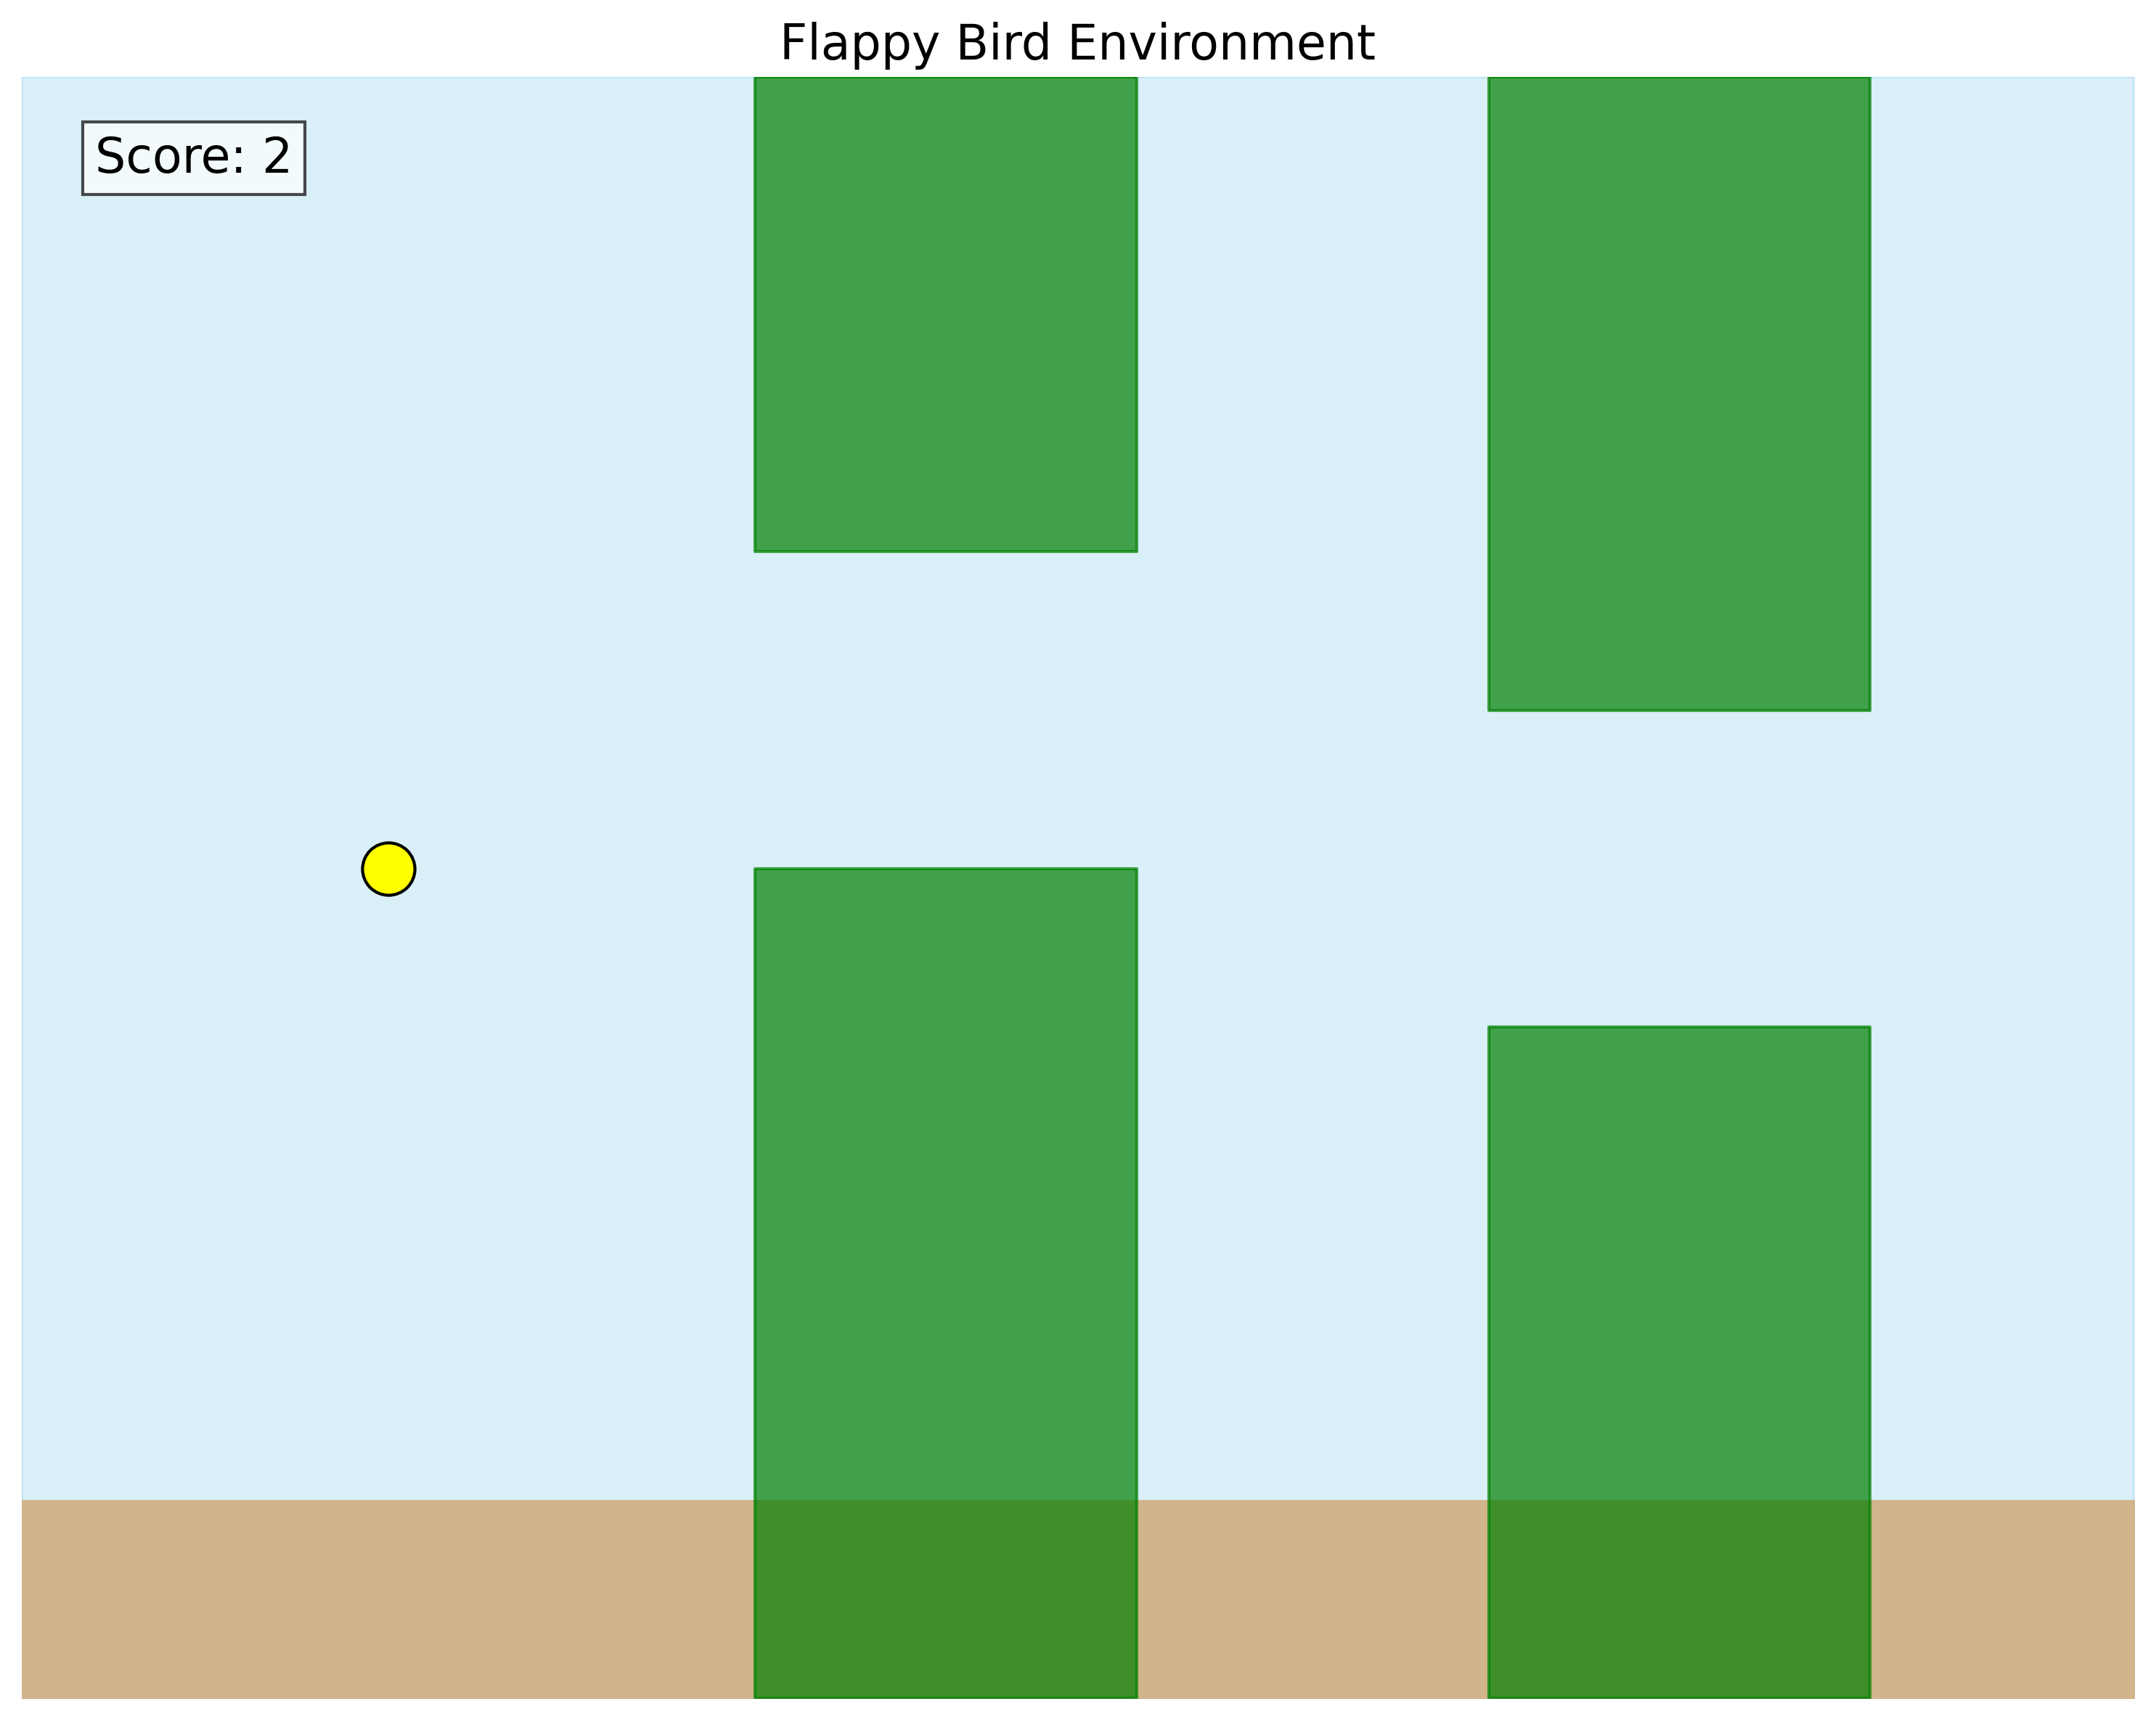
\includegraphics[width=\columnwidth]{/Users/admin/GitHUb/Flappy_Bird_RL/Flappy_Bird_RL/Figures/flappy_environment.png}
\caption{Screenshot of the Flappy Bird environment showing the bird navigating through pipes. The bird's position and velocity are represented, along with the pipe gaps that the agent must navigate.}
\label{fig:flappy_environment}
\end{figure}